
\chapter{Développement d'une méthode d'imagerie cardio-vaculaire sang blanc 3D associant une séquence à temps d'écho ultra-court à l'injection d'un agent de contraste à base de nanoparticule de fer.}
\setlength{\footskip}{50pt}
\chaptermark{Angiographie cardiaque UTE}
\label{Chap4}
\section{Contexte}


L’IRM est devenue un outil de référence pour l’imagerie cardio-vasculaire car elle peut permettre d’obtenir de manière non-invasive des informations anatomiques mais aussi fonctionnelles du coeur. L’imagerie cardiaque résolue dans le temps (appelée imagerie ciné)  s’est donc fortement développée que ce soit chez l’homme ou le petit animal. 
Aujourd'hui les examens de routine sont réalisés en imagerie sang blanc 2D, multi-coupes. Cependant, ce type d'acquisition ne permet pas d’obtenir une résolution importante dans la direction de coupe. Elles peuvent sous-estimer des défauts de contraction du myocarde ou donner des informations sur la fraction d’éjection peu précises, en particulier pour des cas pathologiques entraînant des modifications de la paroi du myocarde \cite{Friedrich:2000aa}. De plus, elles nécessitent un positionnement précis des coupes d'imagerie qui peut s'avérer complexe, notamment chez le petit animal.

Le passage à l'imagerie 3D-t pour des applications cardiovasculaires a donc un intérêt considérable. Cependant, celui-ci est confronté au faible contraste-sur-bruit entre le sang et le myocarde induit par la saturation des spins du sang à l'intérieur des cavités cardiaques avec les séquences traditionnelles d'imagerie cardiaque de type écho de gradient. 
De nouvelles stratégies ont été employées pour obtenir de meilleurs rapports signal-sur-bruit et contraste-sur-bruit. Celles-ci se basent sur l’utilisation des séquences de type “Balanced Steady-State Free Precession” (bSSFP) qui permettent d’obtenir un meilleur signal des liquides et donc du sang \cite{Nezafat2008Inflow-quantifi}. Cependant cette méthode est sensible aux variations locales de champ magnétique ce qui a pour effet de créer des artéfacts caractéristiques sous forme de bandes noires dans les images. Plus le volume à imager est important, comme c’est le cas en 3D, plus le nombre de bandes noires est important. Cela explique la faible utilisation de ces séquences à des champs magnétiques intenses et en particulier sur le petit animal. Des méthodes de correction de ces artéfacts ont été développées \cite{Bangerter:2004kq} et appliquées à haut champ magnétique pour l’imagerie cardiaque \cite{Miraux:2008sf}.  Cependant, ce type de méthode requiert un temps d’acquisition quatre fois plus important \cite{Miraux:2008sf}. 
Une autre approche possible est l'utilisation de séquence sang noir qui permettent d'obtenir des mesures plus précises de l'anatomie cardiaque \cite{Berr2005Black-blood-gra}. En effet, les images sang noir ne sont pas sensibles aux artéfacts de déphasage de flux qui provoque des incertitudes sur les mesures anatomiques en particulier durant la phase systolique. Néanmoins, cela se fait au détriment du rapport signal-sur-bruit, et nécessite par ailleurs d’augmenter le temps d’acquisition des images  \cite{Miraux:2009rm}.

En pratique clinique, l’injection d’agents de contraste à base de gadolinium peut être utilisée pour l’imagerie cardiaque résolue dans le temps. En revanche, cette stratégie n’est pas adaptée pour des applications précliniques. En effet le gadolinium, de par son faible poids moléculaire, diffuse facilement dans le compartiment interstitiel ce qui a pour effet de rehausser le signal dans le myocarde et donc de diminuer le contraste avec le sang.

L’utilisation d’agents de contraste à base de nanoparticules de fer (Ultra Small Particle of Iron Oxyde : USPIO) en tant qu’agent de contraste positif restreint au système vasculaire semble être une bonne alternative aux agents à base de gadolinium grâce à leurs temps de demi-vie dans le sang relativement élevés  \cite{Corot:2006fk,Neuwelt:2009aa}. Il a déjà été montré que ce type d’agent de contraste pouvait être utilisé en tant qu’agent de contraste $T_1$ à des champs magnétiques cliniques (1,5T et 3T) pour l’imagerie de premier passage \cite{Li:2005uq}, pour l'imagerie vasculaire \cite{Sigovan:2009aa,Nayak:2014aa} ainsi que pour l'imagerie cardiaque \cite{Amano:2000aa}.

Cependant la plupart des IRM précliniques disponibles utilisent des champs magnétiques supérieurs ou égaux à 4,7T. Hors, à hauts champs magnétiques, l'effet $T_2^*$ provoqué par les USPIOs est important alors que l'effet $T_1$ est pratiquement stable. Cela explique pourquoi les USPIOs sont principalement utilisés en tant qu'agents de contraste négatif chez la souris, hormis quelques travaux \cite{Jung:2014aa,Girard:2011ec,Loubeyre:1997aa} mais ceux-ci sont réalisés à 3T.

Afin de générer un contraste positif à hauts champs magnétiques, différentes stratégies ont été mises en oeuvre (Saturation Off-Résonance (ORS), l'imagerie de susceptibilité ou des méthodes de compensation de gradient). Toutes ces méthodes ont la même limitation, elles utilisent les perturbations du champ magnétique provoquées par les USPIOs. Or, celles-ci ne peuvent être différenciées d'autres sources de perturbation (interface air/tissus, imperfection du champ $B_0$, etc) qui sont plus présents à hauts champs magnétiques et rendent donc leurs applications difficiles dans des études précliniques.

L'alternatives la plus efficace pour limiter la décroissance du signal provoqué par les agents de contrastes à base de nanoparticules de fer est de réduire fortement le temps d'écho des séquence. L'utilisation de séquences à temps d'écho ultracourts (UTE) permet de s'affranchir de l'effet $T_2$ et $T_2*$ des tissus \cite{Tyler2007Magnetic-resona} et d'utiliser efficacement l'effet $T_1$ des USPIOs. Cette approche est prometteuse pour des applications \textit{in vivo} en particulier dans le champs de l'imagerie quantitative \cite{Girard:2011ec,Gharagouzloo2015Quantitative-co}.


Dans ce chapitre, nous montrerons qu'en combinant l'utilisation d'une séquence 3D UTE (TE < 0.050 ms) et l'injection d'USPIO il est possible d'obtenir un contraste positif quel que soit la valeur du champ  magnétique (4,7T, 7T et 9,4T) ainsi qu'avec une large gamme de concentrations d'USPIO injectés. A partir de ce principe nous montrerons qu’il est possible, grâce à un schéma d’acquisition original d’obtenir, à partir d’un même jeu de donnée acquis, des images 3D+temps de tout le système cardio-vasculaire soit avec une forte résolution spatiale, soit une forte résolution temporelle.


\section{Angiographie rehaussée par un agent de contraste à base de nanoparticules de fer}

\subsection{Agent de contraste}

Les agents de contraste à base de particules de fer sont séparés en plusieurs catégories en fonction de leurs tailles. Les USPIOs ont une taille inférieure à 50 nm. Ils sont composés d’un noyau cristallin d’oxyde de fer entouré d’un “coating” (enrobage généralement composé de dextran) qui évite leur agrégation dans l’organisme. Les USPIOs sont généralement captés par le foie et la rate après une injection par voie intraveineuse. Une des propriétés qui est intéressante pour l'imagerie cardiaque est leur longue durée de demi-vie plasmatique (de à 24 à 36 heures chez l'humain et d'environ 2 heures chez la souris).

Durant ce projet, plusieurs type d'USPIOs ont été utilisés : 
\begin{enumerate}
\item Le Sinerem \textregistered \ (Guerbet, France) : il s'agit d'un dérivé du ferumoxtran-10 possèdant un petit diamètre hémodynamique (30 nm) et un long temps de rémanence vasculaire. Celui-ci est extrêmement espèce dépendant (Demi-vie plasmatique de 36 heures chez l'homme, de 6 heure chez le lapin, de 2 heures chez le rat). Le ferumoxtran-10 est complètement dégradé dans les lyposomes des macrophages en sept jours. Celui-ci a été autorisé sur le marché européen pour la détection des métastases des ganglions lymphatiques.

\item Le P904 (Guerbet, France) : il s'agit un agent de contraste prototype préclinique mis en place pour l'imagerie des macrophages, l'imagerie cellulaire ou l'angiographie. Sa demi-vie plasmatique est également espèce dépendante (Chez la souris : 60 minutes, chez le rat : 145 minutes).
\end{enumerate}

\subsection{Relaxivités}

Les relaxivités $r_1$ et $r_2$ de ces deux agents de contrastes évoluent de façon équivalentes en fonction du champ magnétique. Avec l'augmentation de celui-ci, la valeur de $r_1$ reste quasi-constant et la valeur de $r_2$ va augmenter fortement. Les valeurs de $r_1$ et $r_2$ mesurées pour le Sinerem dans une solution saline sont respectivement de $1,14 \pm 0,06 \ mM^{-1}.sec^{-1}$ et $36,46 \pm 3,03 \ mM^{-1}.sec^{-1}$ à 4,7T; $1,13 \pm 0,09 \ mM^{-1}.sec^{-1}$ et $65,21 \pm 4,23 \ mM^{-1}.sec^{-1}$ à 7T; $1,14 \pm 0,1 \ mM^{-1}.sec^{-1}$ et $86,23 \pm 3,81 \ mM^{-1}.sec^{-1}$ à 9,4T

Les résultats présentés dans la suite du chapitre ont été obtenus avec l'injection du Sinerem mais des résultats équivalents ont aussi été obtenus avec le P904 sa relaxivité étant proche de celle du Sinerem.

\subsection{Contraste positif en fonction du champ magnétique et de la concentration}

Pour évaluer l'effet de l'agent de contraste sur les images, une séquence 3D UTE (TE = 0,031 ms) a été utilisée sur des souris injectées avec 3 valeurs de concentrations de Sinerem (contrôle, 100, 200 et 500 $\mu$mol de fer/kg) pour obtenir des images sur une zone allant du foie au cou ainsi que sur des souris avant injection. Ces valeurs de concentrations ont été choisies car elles correspondent à une gamme de concentration allant des valeurs utilisées pour l'injection chez l'humain aux valeurs de concentration utilisées pour le ciblage cellulaire.
Les paramètres des séquences ont été fixés pour obtenir une résolution de $(234 \ \mu m)^3$ isotropique et pour un temps d'acquisition de 3 min 51 sec.

Des images, sans synchronisation cardiaque et respiratoire, pré et post-injection obtenues à 9,4 T sont montrées dans la figure \ref{fig:UTEConcen}.  Avant l'injection de l'agent de contraste, les vaisseaux sanguins et le sang dans les cavités du coeur ne sont pas facilement identifiables par rapport aux tissus adjacents.

\begin{figure}[H]
\centering
\line(1,0){400} \\
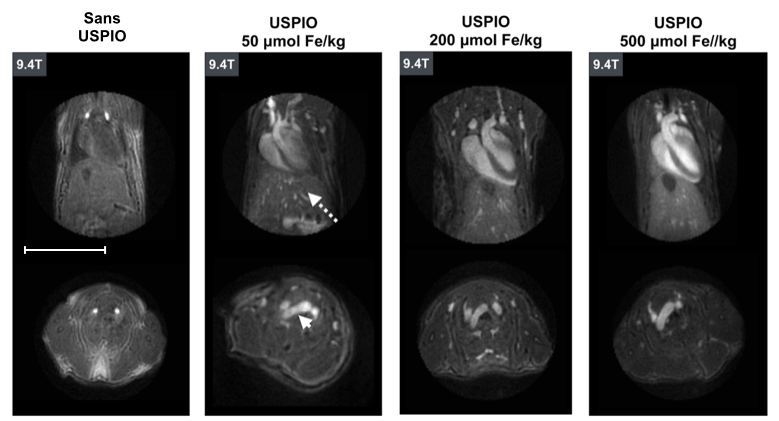
\includegraphics[scale=0.55]{./figure/chap4/Fig_2.png}
\caption[Images obtenues avec une séquence UTE en fonction de la concentration d'USPIO injecté.]{\label{fig:UTEConcen} \textbf{Images obtenues avec une séquence UTE en fonction de la concentration d'USPIO injecté.} Images obtenues sur le coeur et le foie de souris avec une séquence 3D UTE à 9,4T. Les images ont été obtenues avant et après injection d'agents de contraste à différentes concentrations (100, 200 et 500 $\mu$mol Fe/kg), sans synchronisation cardiaque ou respiratoire. La barre d'échelle mesure 15 mm  }
\line(1,0){400} \\ 
\end{figure}

Après l'injection de l'agent de contraste, le sang dans les vaisseaux est visible avec la séquence UTE avec un signal intense et ce quelle que soit la dose injectée. Ce signal est très homogène même dans les zones avec de forte turbulence comme la crosse aortique indiqué par la flèche blanche ou dans les vaisseaux avec un faible débit comme les veines jugulaires. Peu d'artéfacts de flux ou de mouvements sont observés ce qui s'explique par la trajectoire radiale (voir la section \ref{subsec:MouvEtFlux}) ainsi que par le faible TE et l'absence de déphasage des spins par les gradients avant la lecture du signal.

Des observations similaires ont été faites à 4,7 et 7T. Des valeurs de contraste-sur-bruit ont été mesurées entre le sang (dans la crosse aortique et les veines jugulaires) et les muscles et sont répertoriées dans la figure \ref{fig:contraste-sur-bruitUteFlash}. On observe avec la séquence UTE un contraste-sur-bruit d'environ -2 avant injection et une augmentation importante de celui-ci après injection permettant d'obtenir des valeurs toujours supérieures à 18. Cette augmentation est fonction de la dose injectée et la plus forte concentration permet d'obtenir un contraste-sur-bruit supérieur à 40. Cette observation s'explique par le fait que la séquence UTE est peu impactée par l'augmentation du $T_2^*$ grâce à son TE ultracourt, au contraire son signal augmente grâce à l'effet $T_1$ des USPIOs.
Le deuxième point à noter est que le signal diminue aussi avec l'augmentation du champ magnétique pour chaque concentration, cela peut s'expliquer par l'augmentation des valeurs de relaxivité $r_2*$. Cependant cette diminution est très faible et n'est pas significative sur nos mesures.

\begin{figure}[H]
\centering
\line(1,0){400} \\
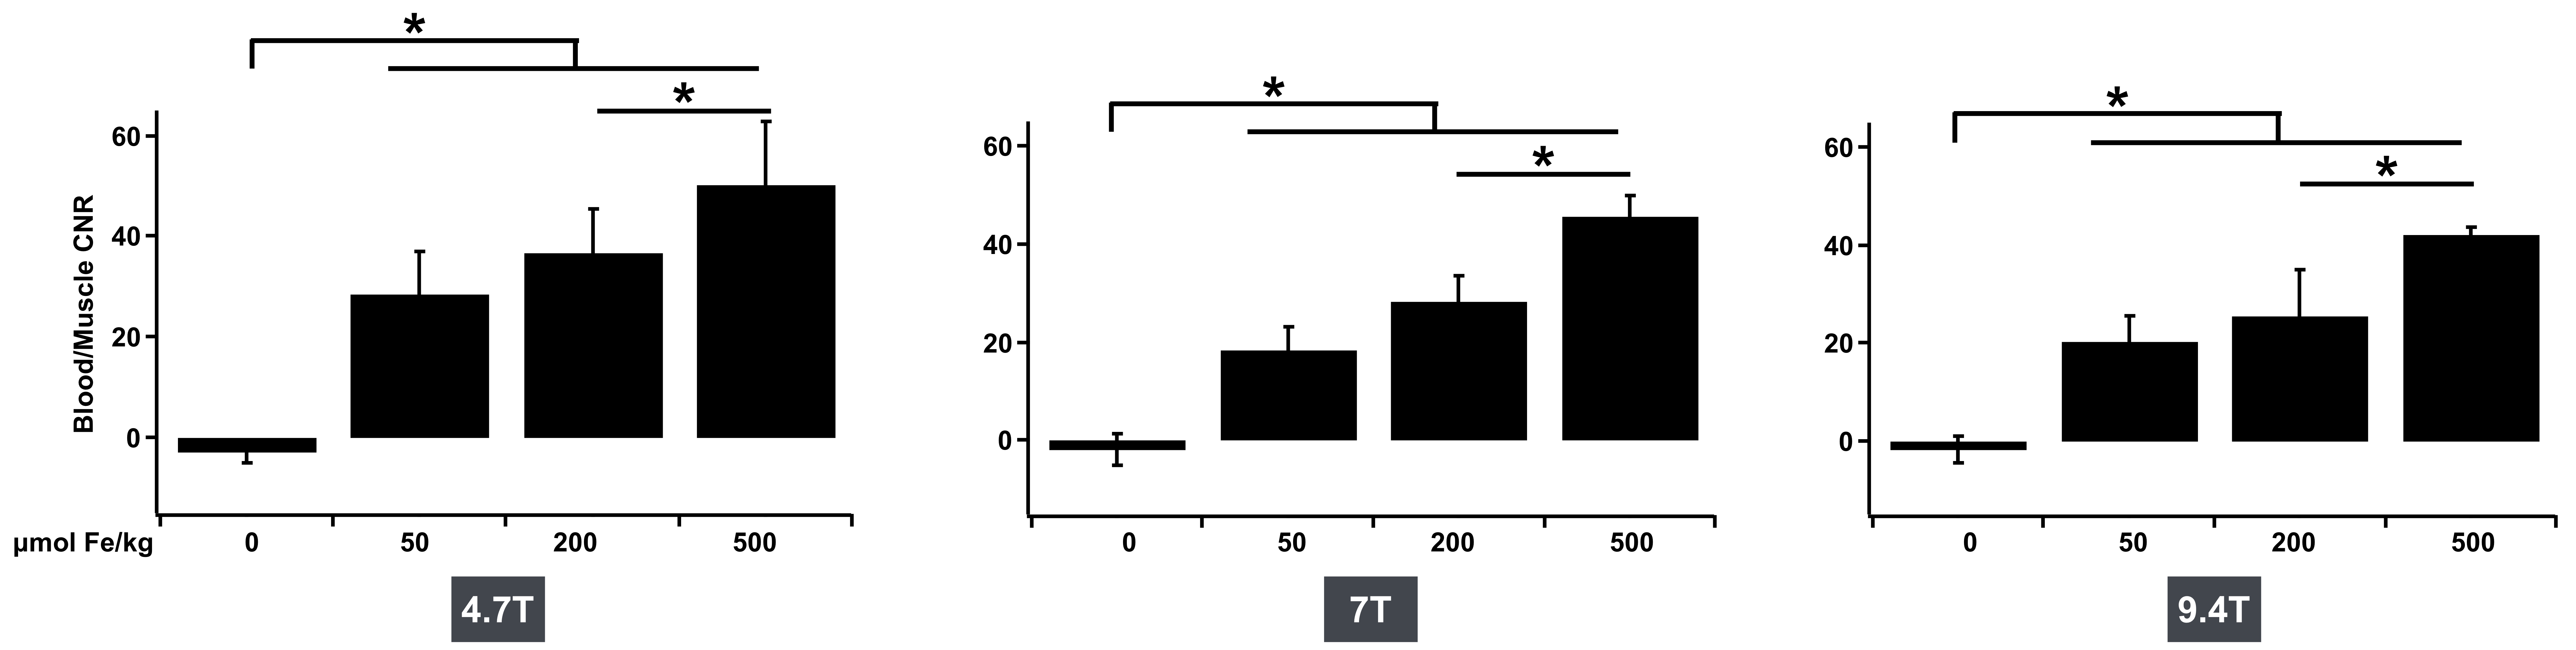
\includegraphics[scale=0.22]{./figure/chap4/Fig_3.png}
\caption[Quantification du rapport contraste sur bruit.]{\label{fig:contraste-sur-bruitUteFlash} \textbf{Quantification du rapport contraste sur bruit.} Mesure du rapport contraste-sur-bruit entre la crosse aortique et le muscle obtenue avec une séquence UTE avant et après injection d'USPIO à 4,7 T, 7 T et 9,4 T et pour différentes concentrations injectées (100, 200 et 500 $\mu$mol Fe/kg). Les valeurs de p inférieures à 0,05 sont indiquées par des astérisques.}
\line(1,0){400} \\ 
\end{figure}

Il est a noté que pour la plus faible concentration de Sinerem injectée (50 $\mu$mol Fe/kg), le contraste varie au cours des expériences : celui-ci a tendance à diminuer d'environ 30 $\%$ au bout d'une heure. Au contraire, les mesures de contraste-sur-bruit restent stables pendant cette période avec les deux concentrations supérieures. 

Tous ces points font de la méthode d'imagerie combinant l'injection d'USPIO et l'utilisation d'une séquence UTE une stratégie envisageable pour l'angiographie 3D et en particulier l'imagerie cardiaque.

\section{Angiographie cardiaque 3D résolue dans le temps}

Au vu du très bon signal obtenu sur les images précédentes, il a donc été envisageable de développer une séquence 3D résolue dans le temps. Cependant l'application de la méthode ciné à la séquence UTE nécessite trop de temps d'acquisition si l'on souhaite obtenir des images respectant le critère de Nyquist. Par exemple, pour des images avec une matrice $(128)^3$, il serait nécessaire de recueillir 102943 projections ce qui correspondrait à un temps d'acquisition de 257 minutes chez une souris anesthésiée avec un rythme cardiaque à 450 battements par minute. Il est possible de sous-échantillonner l'acquisition d'un facteur 2 en impactant peu la résolution mais cela n'apparaît pas suffisant.
Un des avantages des séquences UTE est qu'elles possèdent un faible TR. Il est donc possible de recueillir de nombreux signaux IRM (au moins 40) entre deux battements de coeur. Des signaux peuvent être regroupées pour diminuer le temps d'acquisition mais en limitant le nombre d'images résolues dans le temps qui seront reconstruites. 
Cependant, cette méthode nécessite de modifier la séquence pour que les signaux recueillis successivement ne suivent pas les mêmes trajectoires.


\subsection{Séquence}

Une séquence UTE a donc été développée permettant d'obtenir un nombre d'images ciné (NCine) dont un nombre de signaux IRM recueillis successivement, noté NRegroup, seront regroupés pour reconstruire une image ciné. Dans les expériences chez la souris les paramètres ont généralement été fixés à NCine = 10 et NRegroup = 4. Cela correspond donc à une acquisition de $10 \times 4 = 40$ signaux de décroissance de précession libre (FIDs) à recueillir entre deux battements. Ces paramètres peuvent être adaptés en fonction du rythme cardiaque de l'animal ainsi que du TR de la séquence. Par exemple, avec des TRs de 2 ms pour une souris présentant un intervalle de 140 ms entre deux ondes R de l'ECG, il est donc théoriquement possible de recueillir 70 signaux et de les regrouper par groupe de 7 pour reconstruire 10 images ciné et accélérer la séquence d'un facteur 7.

La séquence développée est présentée dans la figure \ref{fig:SeqUTEUSPIO} avec pour paramètres NCine = 10 et NRegroup = 4. Les différentes projections radiales sont acquises en partant d'une première projection verticale orientée selon z puis s'écartent progressivement de z en tournant autour de ce dernier décrivant ainsi une spirale sur le pourtour de l'espace de Fourier (sphérique) \cite{Saff1997}.
 La position des projections est définie par :
%La trajectoire utilisée pour positionner les projections est une spirale qui part en haut de l'axe Z et termine en bas en tournant autour de l'axe \cite{Saff1997}.
\begin{equation}
\begin{split}
	& Pour \ 1 \leq k \leq NPro : \\ 
	& h_k = -1+\frac{2(k-1)}{NPro-1} \\
	& \Theta_k = arcos(h_k) \\
	& \\
	& \Phi_1=\Phi_N=0 \\	
	& for \ 2 \leq k \leq N-1 \\
	& \Phi_k=\left( \Phi_{k-1}+\frac{3,6}{\sqrt{NPro\times (1-h_k^2)}} \right)mod(2 \pi)	
\end{split}
\end{equation}
où NPro correspond au nombre de projections choisi pour parcourir un espace de Fourier complet. La méthode de répartition des trajectoires permet de les répartir de manière uniforme dans une sphère et ce quel que soit le nombre NPro défini. Cependant dans le cadre de cette séquence NPro doit être un multiple de NRegroup pour regrouper les projections ensembles afin de former une image.

\begin{figure}[H]
\centering
\line(1,0){400} \\
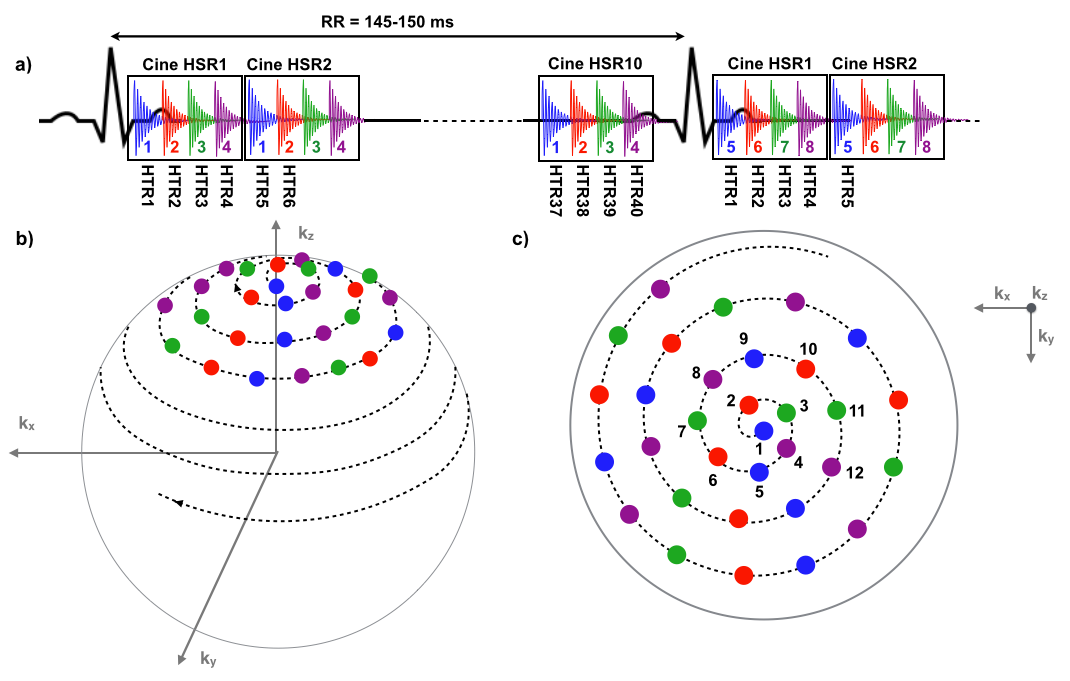
\includegraphics[scale=0.5]{./figure/chap4/SeqUTEUSPIO.png}
\caption[Schéma d'acquisition de la séquence 3D UTE synchronisée sur le rythme cardiaque.]{\label{fig:SeqUTEUSPIO} \textbf{Schéma d'acquisition de la séquence 3D UTE synchronisée sur le rythme cardiaque.} La séquence est représentée avec NCine = 10 et NRegroup = 4. a) Représentation des projections recueillies selon une trajectoire indiqué par le nombre en couleur et servant à remplir des espaces de Fourier indiqué par le terme HTR ou HSR. Les espaces de Fourier HSR correspondent à une reconstruction avec une forte résolution spatiale alors que les espaces de Fourier HTR correspondent à une reconstruction avec une forte résolution temporelle. Les trajectoires sont représentées sur des espaces de Fourier en vue 3D (b) et une vue selon l'axe x-y (c).}
\line(1,0){400} \\ 
\end{figure}

Les NRegroup = 4 premières projections sont recueillies selon des trajectoires différentes  avec dans l'ordre les (n$\degres$ 1,2,3 et 4) comme montré sur la figure \ref{fig:SeqUTEUSPIO}.c. Ce schéma d'acquisition de trajectoire est répété NCine = 10 fois jusqu'au prochain battement de coeur où les 4 trajectoires suivantes (n$\degres$ 5,6,7 et 8) sont alors acquises, NCiné fois, avant de passer aux suivantes, etc.

\subsection{Reconstruction}

\begin{figure}[H]
\centering
\line(1,0){400} \\
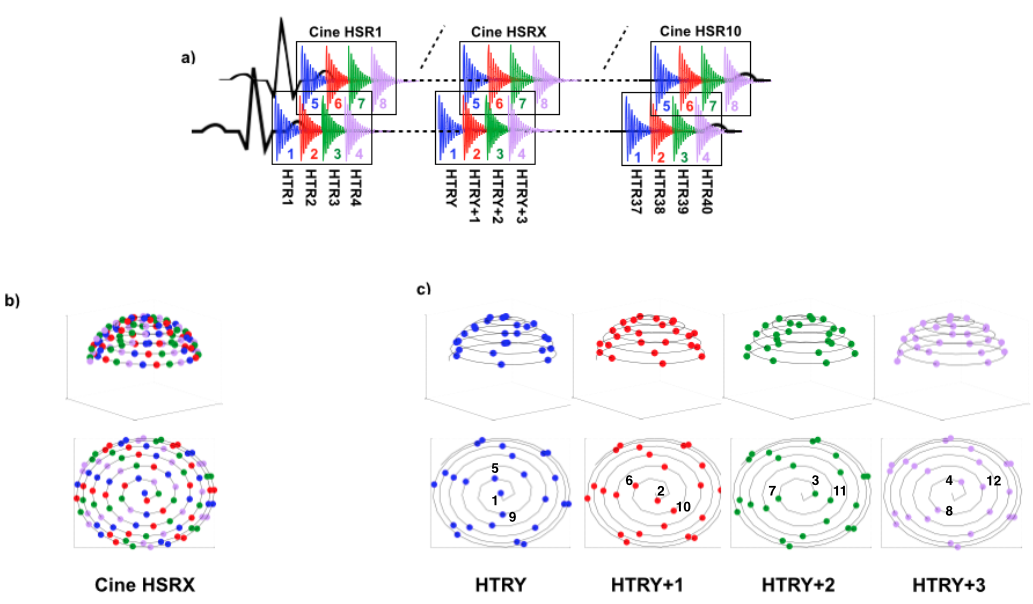
\includegraphics[scale=0.48]{./figure/chap4/RecoUTEUSPIO.png}
\caption[Combinaison et reconstruction des données.]{\label{fig:RecoUTEUSPIO} \textbf{Combinaison et reconstruction des données.} Représentation des projections utilisées pour reconstruire les jeux de données a) haute résolution spatiale et b) haute résolution temporelle.}
\line(1,0){400} \\ 
\end{figure}

Ce schéma d'acquisition permet de reconstruire à partir d'un même jeu de donnée acquis deux types d'images : NCine images avec une forte résolution spatiale (HSR : High Spatial Resolution) ou NCine $\times$ NRegroup images avec une forte résolution temporelle (HTR : High Temporal Resolution). Pour reconstruire les images avec la forte résolution spatiale il faut utiliser toutes les projections recueillies durant la phase Cine HSRX (1245-5678-...) comme indiqué sur la figure \ref{fig:RecoUTEUSPIO}.a et b. L'espace de Fourier reconstruit est donc échantillonné avec NPro projections.
Pour les images avec une forte résolution temporelle, il faut séparer les projections recueillies dans chaque cine HSRX en 4 sous-parties correspondants aux couleurs des projections (voir figure \ref{fig:RecoUTEUSPIO}.a et c) que l'on reconstruira pour obtenir des images avec une résolution temporelle plus importante (NRegroup fois plus grande). Les images reconstruites auront donc une plus faible résolution spatiale car le nombre de projections reconstruites par images ciné sera NRegroup fois plus faible mais les projections seront réparties de manière pratiquement uniforme grâce à la trajectoire utilisée.

\subsection{Imagerie cardiovasculaire résolue dans le temps}

\subsubsection{Acquisition à 4,7T, 7T et 9,4T}

Des images 3D résolues dans le temps ont été recueillies avec une résolution de 156 $\mu$m isotropique pour les 3 champs magnétiques disponibles. La concentration intermédiaire de 200 $\mu$mol de Fe/kg a été injectée pour obtenir les images de la figure \ref{fig:UTEUSPIOField} mais des résultats similaires ont été observés avec la plus forte concentration. Ces images ont été obtenues avec pour paramètres : NCine = 10; NRegroup = 4; NPro = 18144; ce qui correspond à un temps d'acquisition d'environ 12 minutes.

\begin{figure}[H]
\centering
\line(1,0){400} \\
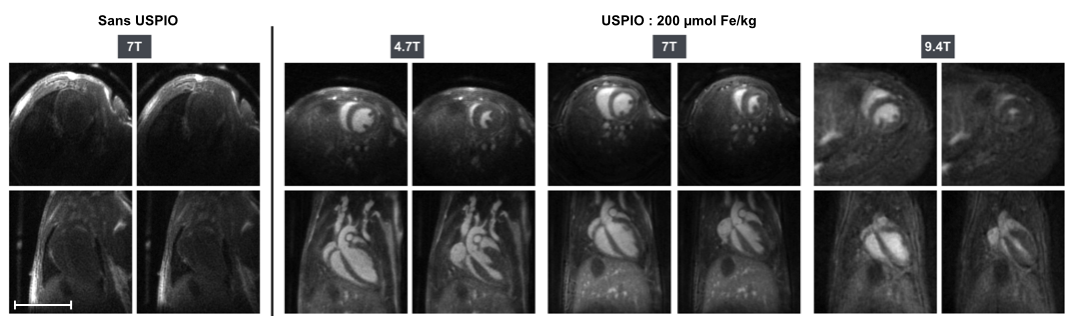
\includegraphics[scale=0.4]{./figure/chap4/Fig_4.png}
\caption[Image résolue dans le temps à plusieurs champs magnétiques.]{\label{fig:UTEUSPIOField} \textbf{Image résolue dans le temps à plusieurs champs magnétiques.} Images 3D obtenues sur un coeur de souris avec une résolution de 156 $\mu$m isotrope à différents champs magnétiques avant et après l'injection d'USPIO à 200 $\mu$mol de Fe/kg. 10 images ont été reconstruites par cycle cardiaque, des images à la fin de la diastole (gauche) et de systole (droite) sont montrées dans deux orientations (En haut : petit axe; en bas : grand axe).}
\line(1,0){400} \\ 
\end{figure}

Des mesures de signal-sur-bruit et contraste-sur-bruit ont été effectuées dans le sang et le myocarde. Le contraste-sur-bruit obtenu avant injection est d'environ -3. Après injection et quel que soit le champ magnétique, un contraste positif est obtenu entre le sang et la paroi du myocarde tout au long du cycle cardiaque (voir les mesures figure \ref{fig:TableMidRes}). Le signal obtenu est très homogène dans les vaisseaux sanguins mais aussi dans les cavités du coeur : le signal mesuré sur les expériences à 7T montre que la déviation standard du signal-sur-bruit mesuré dans le sang des ventricules et la crosse aortique a une valeur comprise entre 1,42 et 2,2 pour un signal-sur-bruit de 70. La qualité des images obtenues à 4,7T et 7T est équivalente. Par contre à 9,4T les mesures de signal-sur-bruit/contraste-sur-bruit sont plus faibles ce qui s'explique par l'utilisation d'une antenne volumique de moins bonne qualité que les antennes surfaciques à 4 éléments utilisées à 4,7 et 7T.

\begin{figure}[H]
\centering
\line(1,0){400} \\
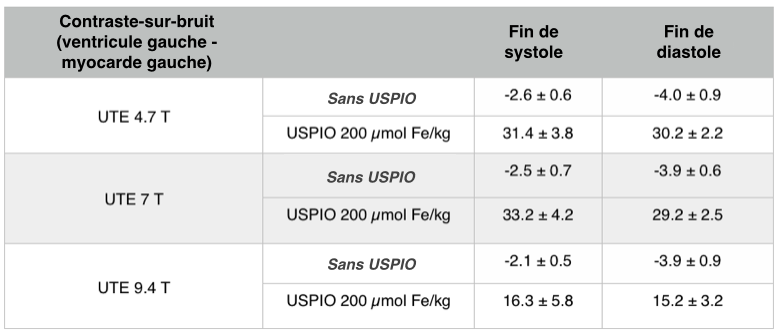
\includegraphics[scale=0.5]{./figure/chap4/TableMidRes.png}
\caption[Tables des mesures de contraste-sur-bruit.]{\label{fig:TableMidRes} \textbf{Tables des mesures de contraste-sur-bruit.} Mesures du contraste-sur-bruit entre le sang dans les ventricules et la paroi du myocarde sur des images obtenues avec la séquence UTE avec une résolution de 156 $\mu$m isotropique à différents champs magnétiques avant et après l'injection d'USPIO à 200 $\mu$mol de Fe/kg.}
\line(1,0){400} \\ 
\end{figure}

\subsubsection{Acquisition haute résolution spatiale et temporelle.}

Des images ont été acquises avec une forte résolution (104 $\mu$m isotrope) à 7T (figure \ref{fig:UTEUSPIOHRS}). Ces images ont été obtenues avec pour paramètres : NCine = 10; NRegroup = 4; NPro = 52540; ce qui correspond à un temps d'acquisition d'environ 35 minutes.
La concentration de l'agent de contraste injecté (200 $\mu$mol de Fe/kg) permet d'obtenir un très bon rapport signal-sur-bruit dans le sang (40,2 $\pm$ 2,3) et un bon contraste-sur-bruit entre le sang et le myocarde (15,8 $\pm$ 2,0) durant la durée de l'expérience.
Cette forte résolution nous permet d'obtenir des mesures de volumétrie précises qui sont en accord avec celles décrites dans la littérature. De plus, elle permet de parfaitement visualiser la déformation de la crosse aortique au cours du cycle cardiaque, de distinguer les valves aortiques (Petite flèche, figure \ref{fig:UTEUSPIOHRS}.a) et de suivre le mouvement des artères coronaires droite et gauche (flèches figure \ref{fig:UTEUSPIOHRS}.b).

\begin{figure}[H]
\centering
\line(1,0){400} \\
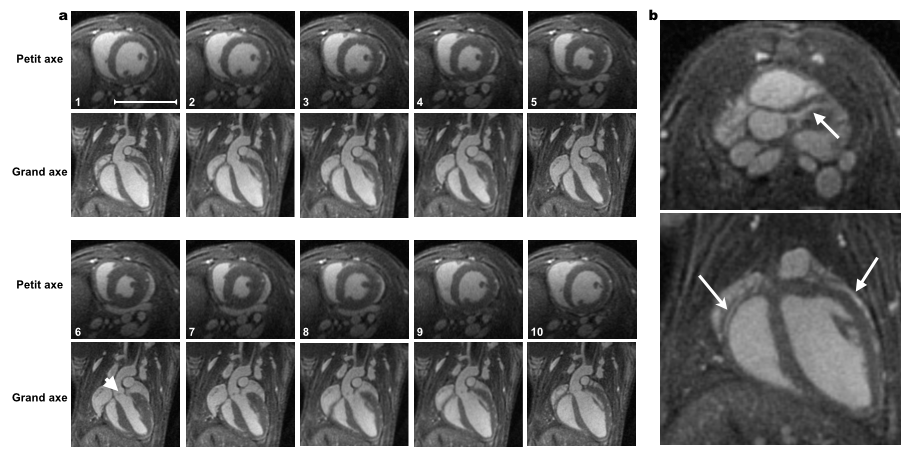
\includegraphics[scale=0.5]{./figure/chap4/UTEUSPIOHRS.png}
\caption[Images haute résolution spatiale.]{\label{fig:UTEUSPIOHRS} \textbf{Images haute résolution spatiale.} a) Images 3D résolues dans le temps au cours du cycle cardiaque (1 image/14 ms), obtenues à 7T avec une résolution isotropique de 104 $\mu$m après l'injection d'USPIO à 200 $\mu$mol de Fe/kg. Le petit axe est représenté dans la lrangée du haut et le grand axe dans la rangée du dessous. La flèche (image 6) indique la valve aortique. b) Images extraites du volume 3D permettant de visualiser les artères coronaires. La barre d'échelle correspond à 1 cm.}
\line(1,0){400} \\ 
\end{figure}

A partir du même jeu de donnée il est aussi possible de reconstruire des images avec une forte résolution temporelle (figure \ref{fig:UTEUSPIOHRT}). Celles-ci permettent de visualiser la déformation du myocarde au cours du cycle cardiaque ce qui peut permettre d'étudier des modèles de trouble de la conduction cardiaque qui induiront un délai dans la contraction. 

Les vidéos des différentes images obtenues sont disponible sur \url{http://www.jcmr-online.com/content/17/1/53/additional}.

\begin{figure}[H]
\centering
\line(1,0){400} \\
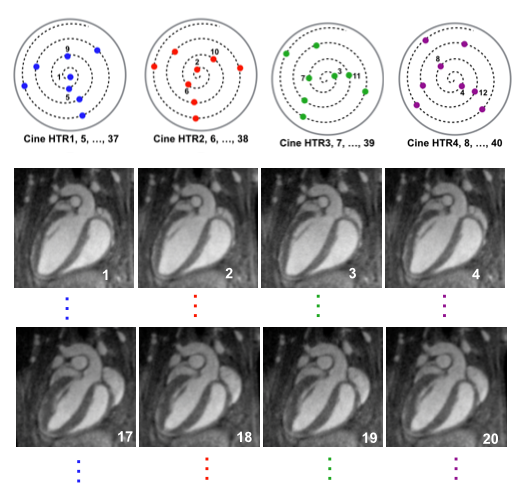
\includegraphics[scale=0.5]{./figure/chap4/UTEUSPIOHRT.png}
\caption[Images haute résolution temporelle.]{\label{fig:UTEUSPIOHRT} \textbf{Images haute résolution temporelle.} Images 3D résolues dans le temps avec une forte résolution temporelle de 3,5 ms.}
\line(1,0){400} \\ 
\end{figure}

\section{Discussion}

Malgré ses nombreux avantages en terme de résolution spatiale, l’imagerie 3D n’est pas la méthode de référence pour étudier le coeur chez le petit animal. En effet, la principale limitation est le temps d’acquisition élevé pour générer ces images, lié à un contraste faible entre le sang et le myocarde. Dans cette optique, une nouvelle méthode d’imagerie cardiaque a été proposée au cours de cette thèse. Elle permet d’obtenir un rapport signal-sur-bruit important ainsi qu’un contraste élevé entre le sang et le myocarde. Ainsi, des images avec des résolutions spatiale et temporelle inégalées ont pu être générées dans un temps d’acquisition de l’ordre de 30 minutes. Le contraste et les résolutions obtenus grâce à cette stratégie sont supérieurs à ceux qui sont décrits dans la litérature en imagerie 4D chez la souris que ce soit en : temps-de-vol \cite{Feintuch:2007aa}, avec l'injection de liposomes remplis de gadolinium \cite{Bucholz:2008uq,Bucholz:2010aa} ou par imagerie sang noir \cite{Miraux:2009rm}.

Pour obtenir un contraste sang blanc en imagerie 3D, le choix s'est porté vers l'utilisation d'agents de contraste à base de nanoparticule de fer. Ils permettent grâce à leur effet $T_1$ de rehausser le signal du sang et grâce à leur longues rémanences vasculaires de générer cet effet pendant une période supérieure à 1 heure. Une alternative possible est l'utilisation d'agents de contraste restreints au domaine vasculaire comme des liposomes chargés au gadolinium \cite{Ersoy:2004aa} mais ces agents n'ont pour le moment pas été approuvés pour des utilisations cliniques et leurs innocuités à long terme n'ont pour le moment pas été validées. Au contraire, de nombreux agents à base de nanoparticules de fer ont déjà été validés pour des injections intraveineuses chez l'humain comme le Sinerem. Leur non-toxicités est donc un avantage pour des études longitudinales chez le petit animal.
Récemment, le ferumoxytol a gagné en intérêt pour des pratiques en IRM clinique \cite{bashir2015emerging} étant donné son autorisation d'utilisation sur le marché des Etats-Unis en tant que complément de fer administré par voie intraveineuse pour des patients avec des anémies provoquées par des maladies chroniques des reins.  De plus, celui-ci dispose d'une forte relaxivité ($r_1= 2 mM^{-1}s^{-1}$) à 7T \cite{Gharagouzloo:2014aa} combiné à une demi-vie plasmatique importante (14-15h) ce qui en fait un agent de contraste extrêmement intéressant pour les IRMs à haut champ magnétique.

Jusqu’à maintenant, les USPIOs n’avaient jamais été utilisés à haut champ magnétique pour de l’angiographie sang blanc car le gain en signal devient de plus en plus faible avec l’augmentation du champ magnétique en utilisant les séquences cartésiennes. De plus, le choix de la dose devenait un problème car la gamme de concentration permettant de ne pas détériorer le signal est aussi de plus en plus restreinte. La solution développée dans ce travail a été l’utilisation d’une séquence radiale à temps d’écho ultracourt qui a permis de négliger l’effet de susceptibilité des nanoparticules. Grâce à cette séquence on observe, \textit{in vivo}, une augmentation du signal en fonction de la concentration injectée d’agent de contraste et ce quel que soit le champ magnétique.

Cette méthode a été utilisée pour de l’imagerie 3D anatomique résolue dans le temps sur le coeur de souris. Toutes les images montrent une très bonne homogénéité du signal sanguin. Ainsi, très peu, voire aucun artéfact de mouvement ou de flux n'a été observé contrairement  aux acquisitions classiques cartésiennes. Ceci est dû à l’aspect radial de la trajectoire UTE mais aussi à l’absence de gradient observé par les spins avant la lecture du signal. Cela permet une mesure extrêmement précise du volume des ventricules contrairement aux séquences d’imagerie sang blanc conventionnelles. Ces séquences peuvent souffrir d’absence de signal sanguin due au déphasage des spins circulants, particulièrement durant les phases systoliques du coeur. 

Le schéma d’acquisition original développé dans ce projet permet, à partir d’un même jeu de donnée, de reconstruire des images ayant une forte résolution spatiale et des images ayant une forte résolution temporelle. Pour ces dernières, il est possible d’obtenir des informations fonctionnelles extrêmement précises sur la contraction du myocarde, mais néanmoins au prix d’une plus faible résolution spatiale provoquée par le sous-échantillonnage des images. Cette méthode d'angiographie est aussi particulièrement adaptée à l'imagerie de grands champs de vue situés au niveau du cerveau ou de l'abdomen (figure \ref{fig:UTEUSPIOAnat}) où les vitesses faibles des flux limitent l'utilisation de séquence temps-de-vol. De plus, l'imagerie de la zone abdominale peut être particulièrement compliquée à cause de la respiration de l'animal ce qui renforce l'utilité de la séquence UTE grâce à sa robustesse au mouvement. 

\begin{figure}[H]
\centering
\line(1,0){400} \\
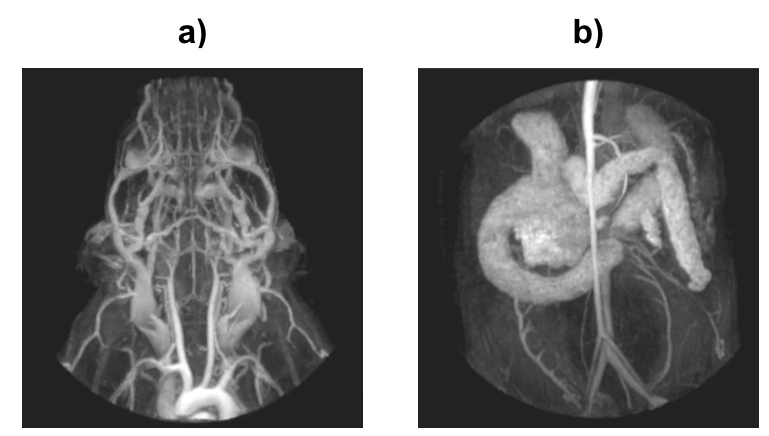
\includegraphics[scale=0.5]{./figure/chap4/UTEUSPIOAnat.png}
\caption[Images anatomiques 3D d'une souris sur différentes zones.]{\label{fig:UTEUSPIOAnat} \textbf{Images anatomiques 3D d'une souris sur différentes zones.} a) s'étendant de la crosse aortique au cerveau; b) abdominal.}
\line(1,0){400} \\ 
\end{figure}

La principale limitation de cette méthode d’acquisition est le fait que ce soit une séquence synchronisée sur le rythme cardiaque. La détection des pics ECG ne pose pas dans ce cas de problème car il y a très peu de changement des gradients d’imagerie, par contre, il est nécessaire de stabiliser le rythme cardiaque de l’animal pendant une durée élevée pour obtenir une image de bonne qualité. Cela peut être un problème pour les séquences permettant d’obtenir des images avec une très forte résolution spatiale car celles-ci peuvent durer plus de 35 minutes. Une solution est d’accélérer la séquence pour réduire la probabilité d’avoir des changements de rythme cardiaque importants. Les méthodes d’imagerie parallèle sont difficilement utilisables en pratique préclinique au vue du faible nombre de canaux des antennes, mais il a précédemment été montré que les séquences radiales sont favorables aux algorithmes de reconstruction de type “compressed sensing”. Ceci est une piste à explorer pour réduire les temps d'acquisitions \cite{Nam:2013nx}.
 
 
Cette méthode est a priori transposable chez l'homme bien qu'il soit nécessaire de l'adapter à d'autres contraintes. En effet, la séquence est ici seulement synchronisée sur le rythme cardiaque. Hors, chez l’humain, les mouvements respiratoires sont bien plus amples et doivent être corrigés.
Un deuxième point important est que la dose utilisée dans cette étude est supérieure à celle généralement injectée chez l'humain. En l'absence d'information supplémentaire, il n'est pas possible aujourd'hui d'utiliser de telles concentrations chez le patient. Cependant, des doses entre 50 et 100 $\mu$mol de Fe/kg combinées à la séquence 3D UTE devraient tout de même permettre d'obtenir, particulièrement à des champs $\leq$ à 3T, des images du système vasculaire chez l’humain avec des résolutions temporelles et spatiales supérieures à celles obtenues pour le moment en pratique clinique. Le dernier point problématique à étudier est le temps d’acquisition important de cette séquence supérieur à 30 minutes, qui sera augmenté dans le cas d’une correction de la respiration. Celui-ci pourra être réduit grâce au facteur d’acceleration important pouvant être obtenue en imagerie parallèle. De plus, grâce aux TR particulièrement court pouvant être utilisé pour cette séquence, il est possible d’associer les projections proche temporellement dans la même image ciné et ainsi accélérer l’acquisition \cite{Trotier2015Time-resolved-T}.
Enfin, il apparaît particulièrement intéressant de développer, à la fois en préclinique et en clinique, les techniques d’auto-synchronisation permettant de s’affranchir de l’utilisation de capteurs ECG et de choisir a posteriori la résolution temporelle des images. Ces technique sont tout à fait compatibles avec les méthodes d’encodage radial.










